\section{Integration with LoRaWAN}
\label{sec:implementation}

% \begin{figure}
%     \centering
%     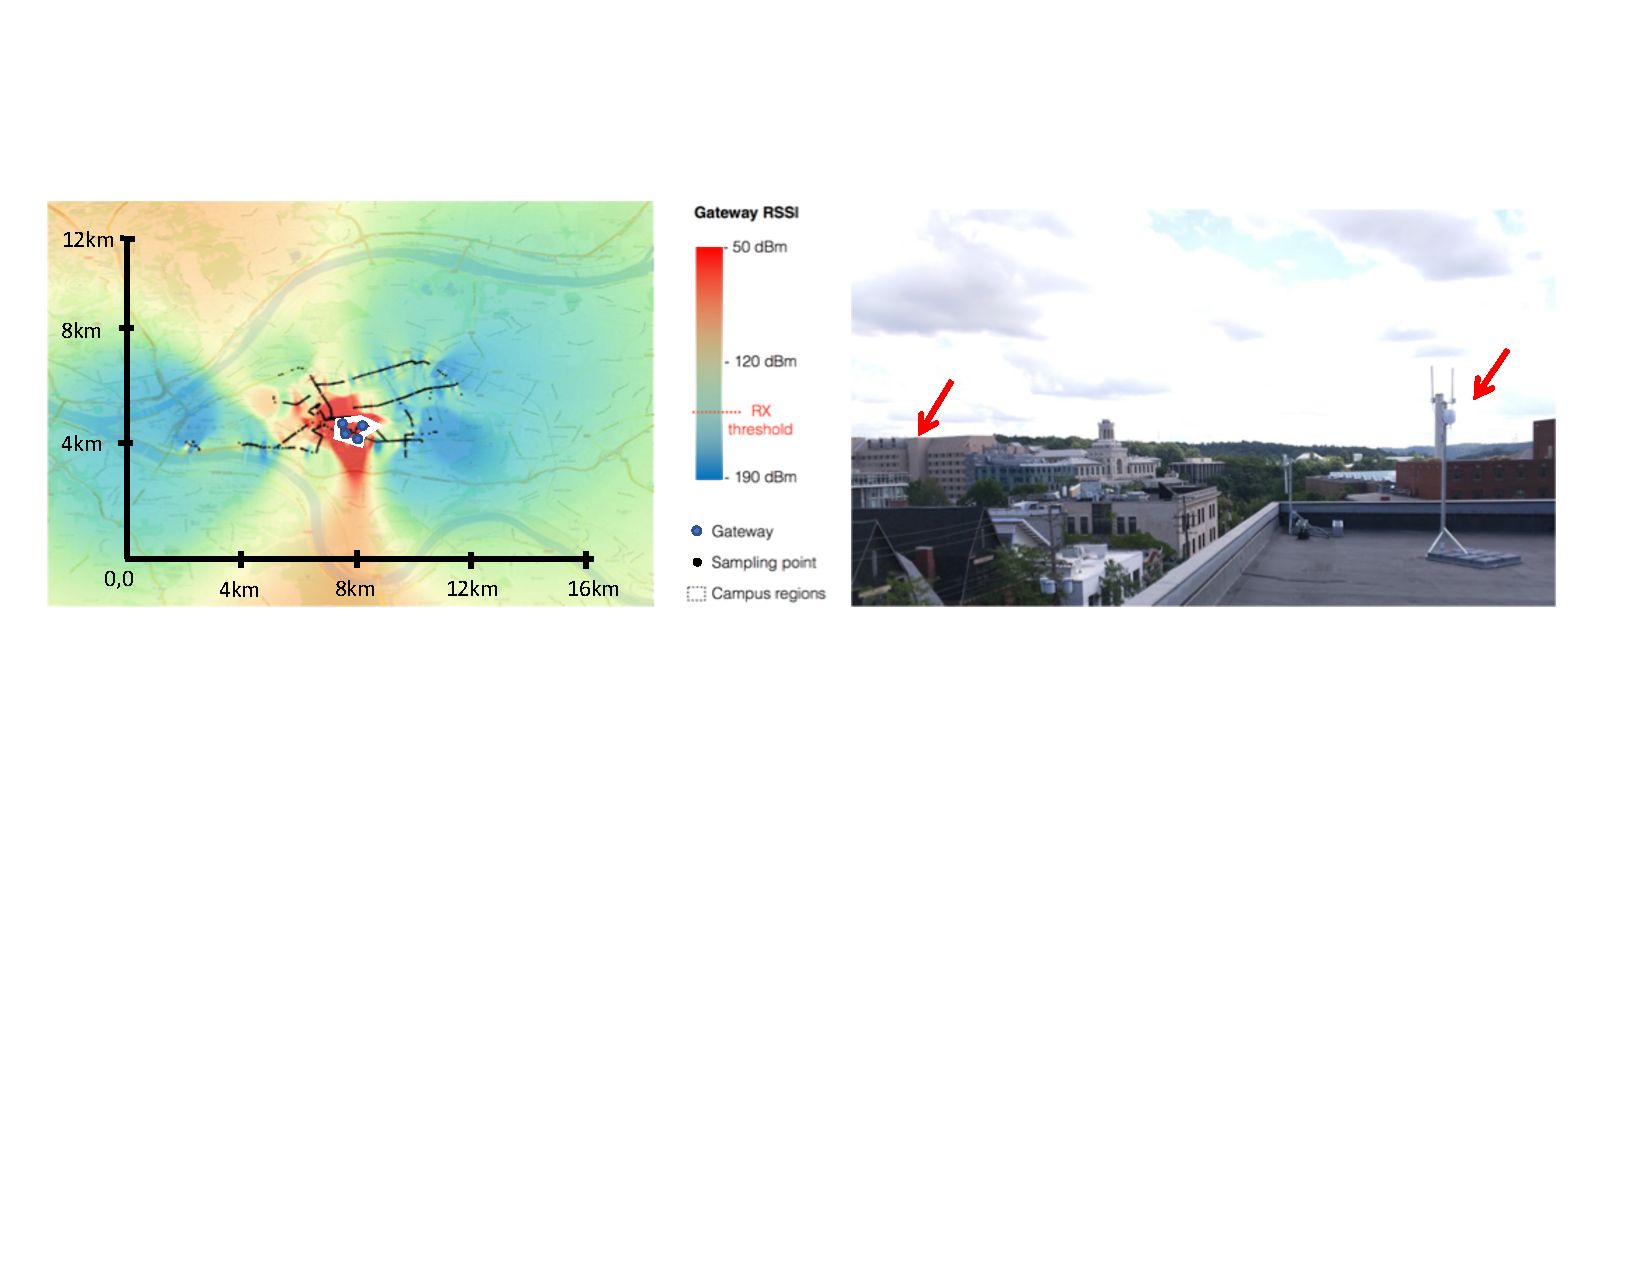
\includegraphics[width=0.45\textwidth]{figures/deployment.pdf}
%     \caption{Deployment photos and coverage heat maps (\textit{Parts of images have been occluded to maintain anonymity})}
%     \label{fig:deployment}
% \end{figure}

\begin{figure}[!htb]
\centering
\begin{tabular}{@{}c@{}}
\subfloat[OpenChirp network coverage heatmap around Pittsburgh]{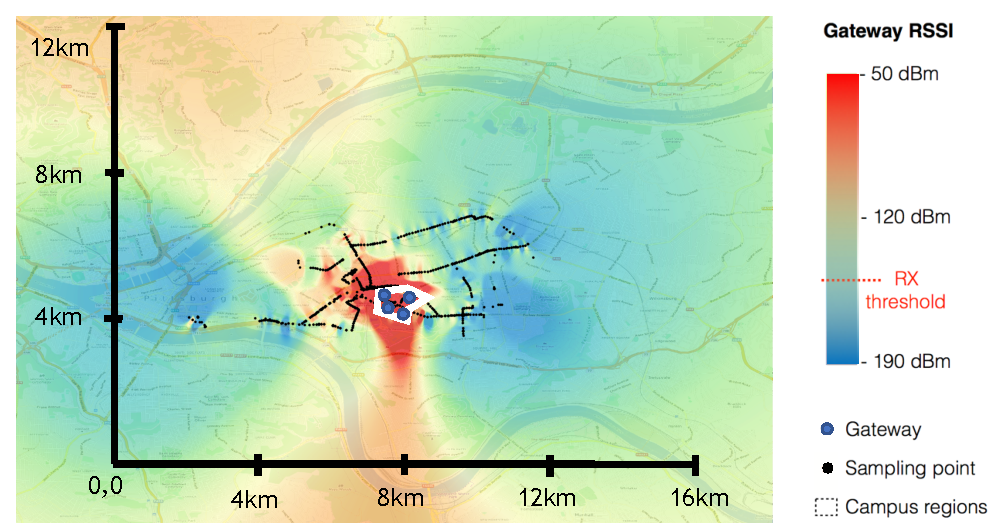
\includegraphics[height=1.2in]{figures/heatmap_openchirp_cropped}
\label{fig:coverage-map}}
\hspace{0.05in}
\subfloat[Rooftop gateway]{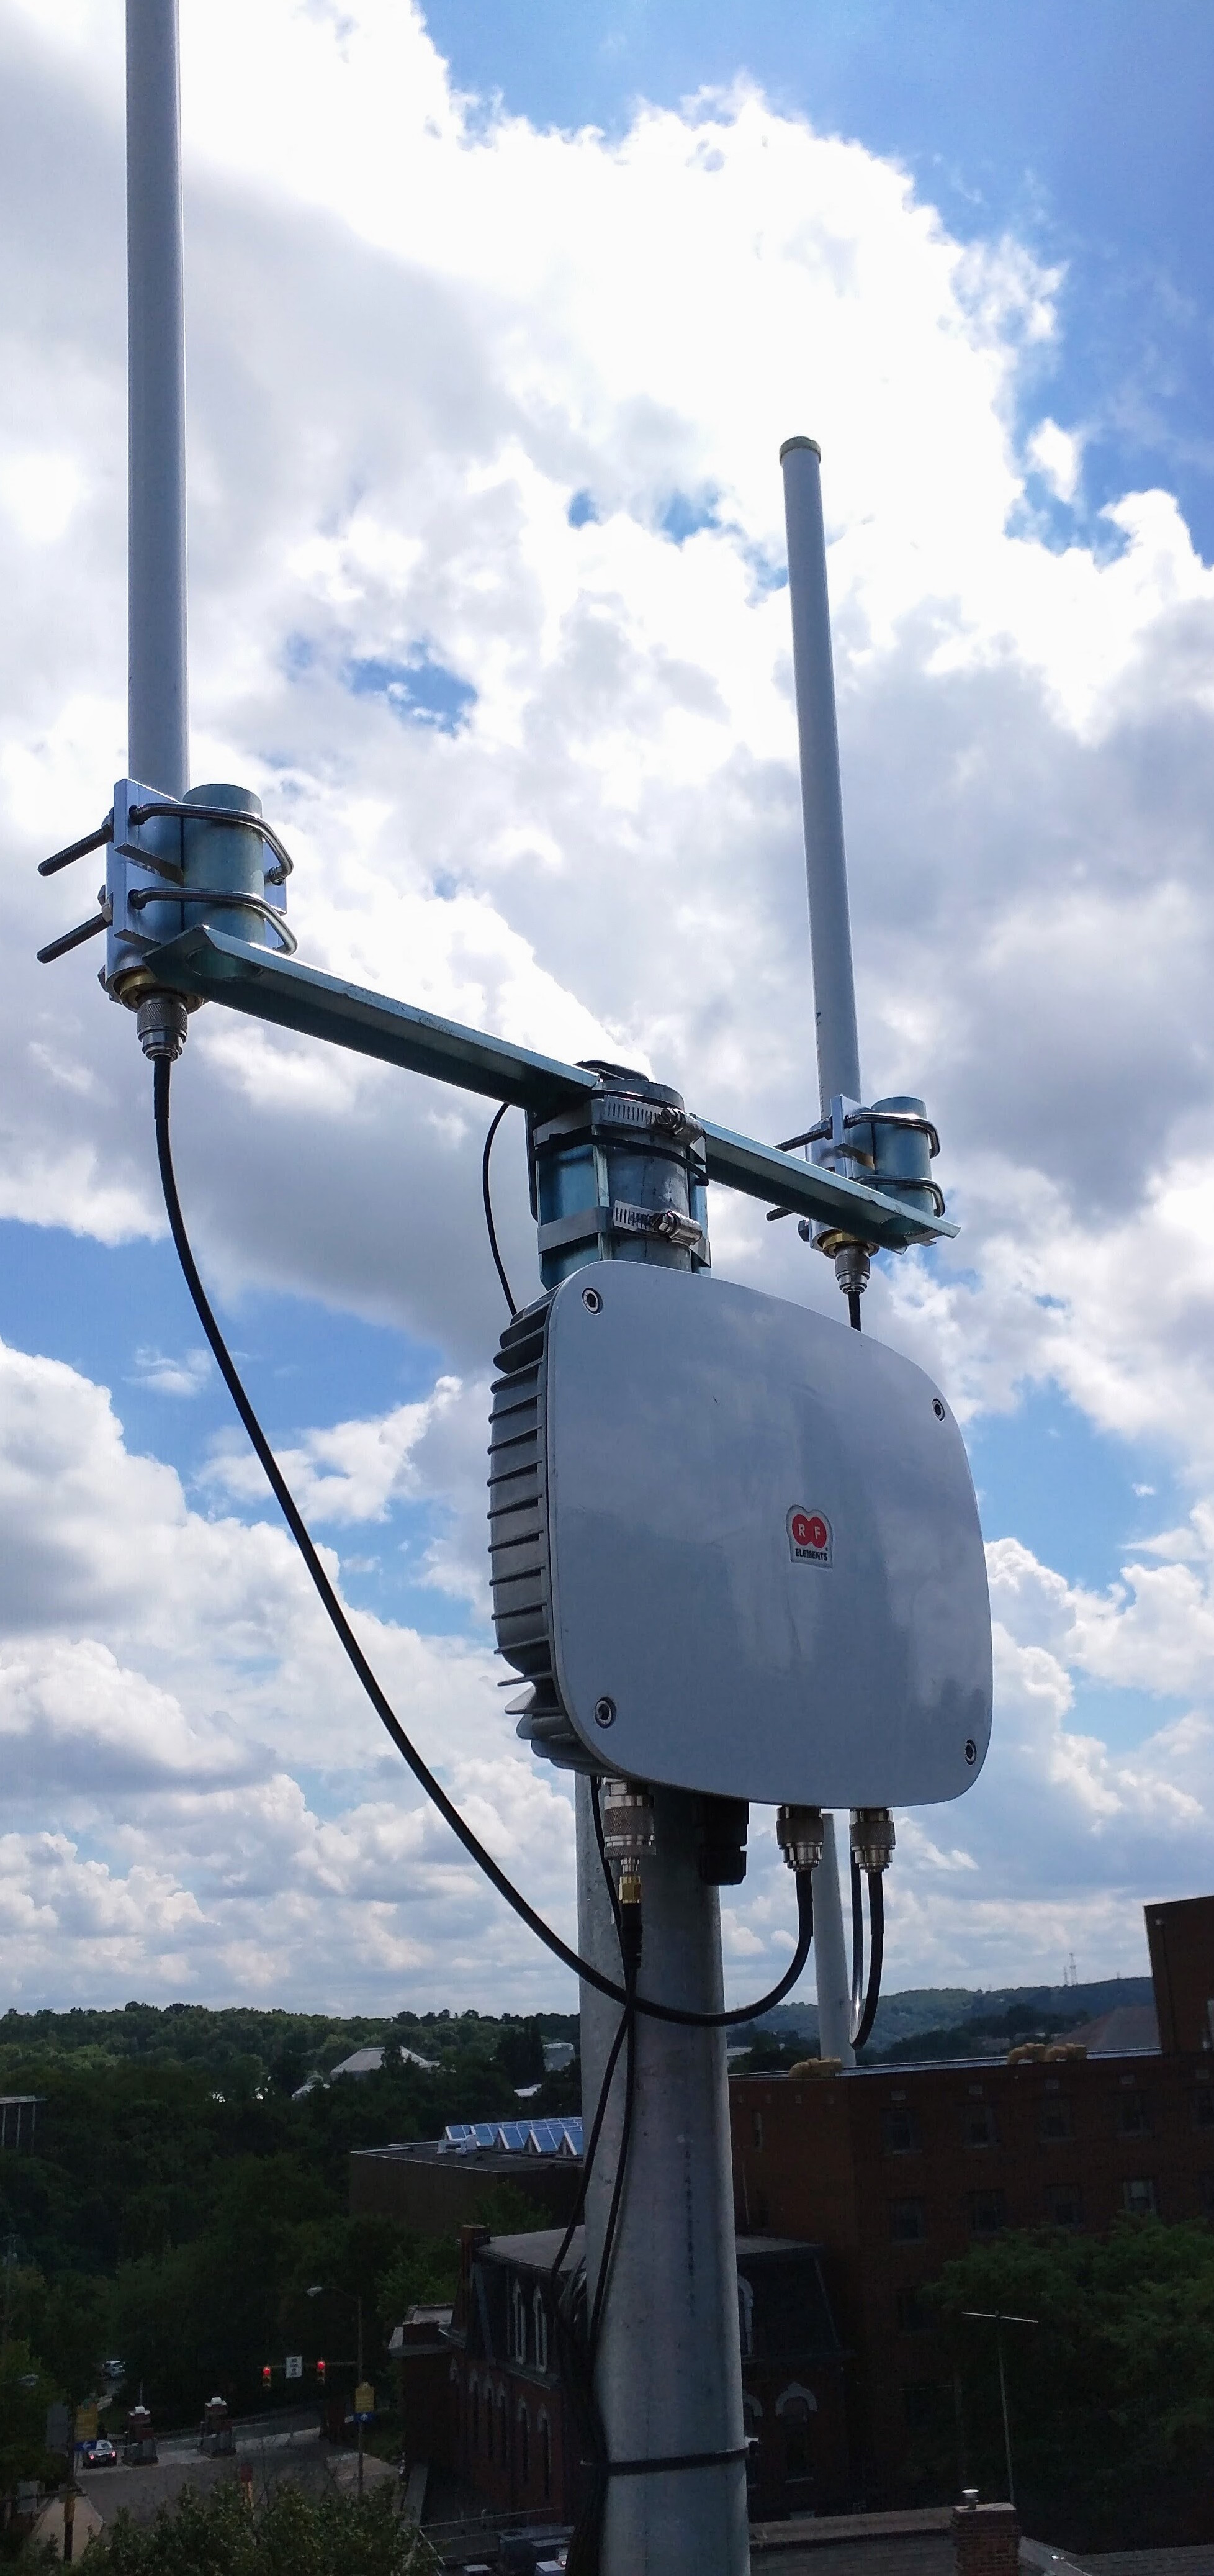
\includegraphics[height=1.2in]{figures/gateway_deployment_cropped}
\label{fig:rooftop-gw}}
\end{tabular}
\caption{}
\label{fig:deployment}
\compactimg
\end{figure}

Charm is implemented as a service running on a campus-wide LoRaWAN network installed at Carnegie Mellon University.  We currently have four gateways mounted on rooftops providing wide area coverage and eight auxiliary indoor gateways extending coverage into remote parts of campus. The LoRaWAN network is powered by the open-source OpenChirp (\url{http://www.openchirp.io}) framework that allows students and faculty to login with their campus accounts and create device endpoints for capturing and sharing data.  OpenChirp provides services that can be attached to data streams that can perform operations ranging from basic data storage to binary-to-JSON packing and unpack. A RESTful interface is used to configure meta-information about devices and set access control privileges that define how other users can interact with data streams.  The only modifications required to make a gateway Charm enabled is the additional hardware platform for receiving raw I/Q streams and a modified LoRaWAN packet forwarder that runs the packet reception event detector, maintains a circular buffer of I/Q streams and brokers interactions with the Charm cloud.  Communication between gateways and the cloud is managed using the OpenChirp's MQTT publish subscriber messaging layer where compressed Charm packets can be easily grouped and organized based on location.  The Charm service can instruct clients to switch to faster data rates (as compared to the normal data rate negotiation process) by spoofing improved SNR values during the join process. In this way, Charm can seamlessly operate with existing LoRaWAN devices with no modification.

\figref{deployment} shows examples of our gateway hardware deployed in the field along with the coverage in and around campus.  The network is currently supporting a wide-range of applications from student projects, study-space monitoring, and building occupancy sensing all the way to mechanical room environmental sensing and utility sub-metering for the campus facilities maintenance team.  The client transmitters in our experiments use the Semtech SX1276 LoRaWAN chipset. The figure also shows an example coverage heat map generated by nodes deployed throughout campus and the neighboring area.  We see that the network with just four outdoor gateways is able to cover almost 10$km^2$ of urban space.

